\appendix

\newtcblisting{strategycode}{
  enhanced,
  listing only,
  breakable,
  width=\textwidth,
  colback=cardbg,
  colframe=accent,
  boxrule=0.35pt,
  arc=2pt,
  left=6pt,
  right=6pt,
  top=4pt,
  bottom=4pt,
  boxsep=0pt,
  listing options={
    language=Python,
    basicstyle=\ttfamily\scriptsize,
    keywordstyle=\color{accent}\bfseries,
    commentstyle=\color{black!55},
    stringstyle=\color{black!70},
    columns=fullflexible,
    keepspaces=true,
    showstringspaces=false,
    breaklines=true,
    breakatwhitespace=true
  }
}
\newpage


\section{Benchmark Object and Task Suite}
\label{app:benchmark-object}

\subsection{Run Protocol and Policy System}
\label{app:protocol-details}

An \evopolicygym{} run gives the agent a live workspace and a fixed interaction
budget for improving one executable policy system. The server stages
\texttt{AGENTS.md}, initializes \texttt{system/} with the policy entry point,
and exposes a local HTTP service. The agent uses \texttt{/info} to inspect the
remaining budget and protocol limits, \texttt{/task} to read the task and
policy contract, and \texttt{/submit} to request visible train rollouts.
Validation, held-out evaluation, and finalization remain server-side.

The policy entry point is \texttt{system/policy.py}. It exports a top-level
\texttt{Policy} class whose constructor receives the observation space, action
space, and environment metadata; the server then calls \texttt{reset} once per
episode and \texttt{act} at each environment step. Agents may add modules,
configuration files, tests, weights, memory files, and analysis utilities under
\texttt{system/}. For each submit, the server imports the submitted policy and
constructs a fresh \texttt{Policy} instance, so durable state lives in files
under \texttt{system/}.

Episode budget is charged by the expanded list of requested train case
indices. In Core16, each run uses a total budget of 128 episodes and allows
between 1 and 128 episodes per submit. The server preserves request order and
repeated indices. Request-format failures are rejected before snapshot and do
not consume budget. Once a request passes protocol validation, the server
snapshots \texttt{system/}; import errors, initialization errors, rollout
timeouts, and other execution-stage failures still consume the requested
episode budget and write visible feedback.

Feedback is written under \texttt{feedback/submit\_NNN/}. Each completed
submit has a \texttt{summary.json} containing status, requested case indices,
remaining budget, episode returns, episode lengths, errors, timing, and
aggregate return statistics. Successful episode directories contain step-level
\texttt{trajectory.jsonl} records, policy stdout/stderr streams, and optional
environment-specific media such as rendered video or external observation
arrays. Submit-level failures write \texttt{errors.txt}; per-episode failures
write the corresponding episode error file while preserving the rest of the
submit evidence when possible.

The workspace has live no-rollback semantics. The agent may overwrite its own
\texttt{system/} files after each submit, and harmful valid edits stay visible
until the agent repairs or restores them. The server separately stores
immutable submitted checkpoints for hidden validation and final held-out
evaluation.

\subsection{Core16 Suite}
\label{app:core16-suite-details}

Core16 selects 16 implemented Gymnasium-compatible scenarios from four
environment families. The suite spans control, visual driving, locomotion,
symbolic partial observability, manipulation, and traffic-style control,
requiring controllers, visual abstractions, world models, phase machines, and
recovery logic.

\begin{table}[H]
\caption{Implemented \evopolicygym{} scenarios used in the 128-episode
Core16 suite.}
\label{tab:suite}
\begin{center}
\scriptsize
\setlength{\tabcolsep}{3.5pt}
\resizebox{\textwidth}{!}{%
\begin{tabular}{llll}
\toprule
Category & Suite ID & Gymnasium env & Obs./action \\
\midrule
Gym / Box2D & \texttt{gym/acrobot} & \texttt{Acrobot-v1} & state/discrete \\
Gym / Box2D & \texttt{gym/continuouscar} & \texttt{MountainCarContinuous-v0} & state/continuous \\
Gym / Box2D & \texttt{gym/bipedal} & \texttt{BipedalWalker-v3} & state/continuous \\
Gym / Box2D & \texttt{gym/racing} & \texttt{CarRacing-v3} & image/continuous \\
MuJoCo & \texttt{gym/reacher5} & \texttt{Reacher-v5} & state/continuous \\
MuJoCo & \texttt{gym/halfcheetah5} & \texttt{HalfCheetah-v5} & state/continuous \\
MuJoCo & \texttt{gym/ant5} & \texttt{Ant-v5} & state/continuous \\
MuJoCo & \texttt{gym/pusher5} & \texttt{Pusher-v5} & state/continuous \\
MiniGrid & \texttt{gymnasium/MiniGrid-DoorKey-16x16-v0} & \texttt{MiniGrid-DoorKey-16x16-v0} & symbolic/discrete \\
MiniGrid & \texttt{gymnasium/MiniGrid-KeyCorridorS4R3-v0} & \texttt{MiniGrid-KeyCorridorS4R3-v0} & symbolic/discrete \\
MiniGrid & \texttt{gymnasium/MiniGrid-FourRooms-v0} & \texttt{MiniGrid-FourRooms-v0} & symbolic/discrete \\
MiniGrid & \texttt{gymnasium/MiniGrid-ObstructedMaze-1Q-v1} & \texttt{MiniGrid-ObstructedMaze-1Q-v1} & symbolic/discrete \\
Robotics / Driving & \texttt{gymnasium/parking-v0} & \texttt{parking-v0} & state/control \\
Robotics / Driving & \texttt{gymnasium/roundabout-v0} & \texttt{roundabout-v0} & state/control \\
Robotics / Driving & \texttt{gymnasium/FetchPush-v4} & \texttt{FetchPush-v4} & dict/continuous \\
Robotics / Driving & \texttt{gymnasium/FetchPickAndPlace-v4} & \texttt{FetchPickAndPlace-v4} & dict/continuous \\
\bottomrule
\end{tabular}
}
\end{center}
\end{table}


The four-by-four organization gives each family equal weight in category-level
analysis while preserving heterogeneous policy interfaces. State-control tasks
test compact feedback interpretation, CarRacing adds visual abstraction,
MiniGrid stresses persistent symbolic state, and the Fetch tasks require
geometric phase control. This mix is why raw returns are reported per
environment and aggregated only after within-environment ranking.

\section{Evaluation Protocol and Agent Configuration}
\label{app:evaluation-protocol}

\subsection{Visibility, Selection, and Scoring}
\label{app:evaluation-and-scoring}
\label{sec:hidden-eval}
\label{sec:scoring-audit}

Each Core16 run uses three disjoint case splits. Train cases are visible as
integer handles and provide all in-loop feedback. Validation and held-out cases
are server-side. For the experiments in this paper, hidden validation contains
16 cases and hidden held-out evaluation contains 32 cases per environment. The
agent never sees validation or held-out case identities, trajectories, returns,
or failure details during optimization.

\begin{table}[H]
\caption{Visibility boundary for agent-facing artifacts.}
\label{tab:visibility}
\begin{center}
\begin{tabular}{lll}
\toprule
Split & Agent-visible during run & Server role \\
\midrule
Train & IDs, summaries, trajectories, failures & Online revision signal \\
Validation & None & Private checkpoint selection \\
Held-out & None & Final generalization measurement \\
\bottomrule
\end{tabular}
\end{center}
\end{table}

After the 128-episode train budget is exhausted, the server evaluates every
\texttt{status == ok} checkpoint on the hidden validation split. The checkpoint
with the highest validation mean return is selected; equal validation means are
resolved by choosing the later submit. The selected checkpoint is then
evaluated on the held-out split. The raw held-out mean return is the
per-environment number reported in Table~\ref{tab:core16-raw}.

Cross-environment aggregation uses only ranks within each environment. Let
$y_{m,e}$ be the held-out mean return for entry $m$ on environment $e$, and
let $\mathrm{rank}_e(m)$ be the descending rank of $y_{m,e}$ among the four
reported agents plus the uniform random-policy reference. For agents,
$y_{m,e}$ is validation-selected; for the random-policy reference, it is the
held-out mean return of uniform random actions on the same 32 held-out cases,
with no training budget or validation selection. Equal held-out means share the
same rank score. The per-environment score is
\[
s_{m,e}=1-\frac{\mathrm{rank}_e(m)-1}{N_e-1},
\]
where $N_e=5$ in the Core16 leaderboard. Category scores average $s_{m,e}$
over the four environments in that category. The Core16 score averages
$s_{m,e}$ over all 16 environments. These aggregate scores are analysis
metrics; hidden validation selection and held-out evaluation operate on raw
environment returns.

This scoring separates two questions. Raw held-out means show how strong a
selected policy is on one environment. Rank-normalized scores summarize which
agent more consistently converts the same interaction budget into competitive
policies across reward scales.

Runs also record audit signals: accepted and rejected submits, budget consumed
per submit, post-hoc validation best-so-far curves, selected checkpoint,
invalid-transition rate, score-drop events, policy complexity growth, wall
time, and agent token accounting when available. These traces support the
behavior analysis in Section~\ref{sec:behavior-analysis}.

\subsection{Agent and Run Configuration}
\label{app:agent-run-configuration}

All four leaderboard agents use the same run-level configuration: the Core16
environment list, a 128-episode train interaction budget, minimum submit size
1, maximum submit size 128, hidden validation size 16, and hidden held-out size
32. Each run uses external train/validation/held-out case files for the
corresponding environment. The server binds to a local loopback address with an
ephemeral port, and the port is exposed to the agent only through the staged
run instructions. The random-policy reference in Tables~\ref{tab:core16-raw}
and~\ref{tab:aggregate} is evaluated directly on the same held-out cases and
does not use this agent harness configuration.

\begin{table}[H]
\caption{Harness configuration for the Core16 leaderboard agents.}
\label{tab:agent-config}
\begin{center}
\footnotesize
\setlength{\tabcolsep}{4pt}
\begin{tabular}{llll}
\toprule
Agent & Harness & Model string & Shared settings \\
\midrule
GPT-5.5 & Codex & \texttt{gpt-5.5} & retries 5, backoff 4.0, bypass enabled \\
Claude Opus 4.7 & Claude Code & \texttt{claude-opus-4-7-thinking-max} & retries 5, backoff 4.0 \\
MiniMax-M3 & Claude Code & \texttt{MiniMax-M3} & retries 5, backoff 4.0 \\
DeepSeek-V4-Pro & Claude Code & \texttt{deepseek-v4-pro} & retries 5, backoff 4.0 \\
\bottomrule
\end{tabular}
\end{center}
\end{table}

The Claude Code-compatible runs expose the same tool profile:
\texttt{Bash}, \texttt{Read}, \texttt{Edit}, \texttt{Write}, \texttt{Glob}, and
\texttt{Grep}, with bypass-style permissions. The Codex run uses the Codex
adapter with a persistent logical session. Retries handle harness or service
timeouts and exceptions; retry events do not add environment interaction and do
not change the server-side budget accounting.

The shared run budget fixes the environment-interaction comparison. Harness
differences still affect context management and tool traces, so token and cost
statistics are diagnostic only and excluded from scoring.

\section{Supplementary Analysis Diagnostics}
\label{app:additional-diagnostics}

This section expands the quantitative diagnostics used in
Section~\ref{sec:behavior-analysis}. The ability table provides the
per-environment values behind the synthesis/tuning split; the token table
describes harness-level context traffic; and the edit-size plot summarizes how
large checkpoint changes relate to visible improvement. These diagnostics
explain behavior but do not affect validation selection, held-out evaluation, or
leaderboard rank.

\subsection{Per-Environment Relative Held-Out Performance by Task Demand}
\label{app:ability-split-detail}

\begin{table}[H]
\caption{Per-environment values behind Figure~\ref{fig:two-abilities}. Scores
are scaled between a random policy ($0$) and the best evaluated agent
performance on that environment ($1$), with random anchors measured on the
same held-out pools.}
\label{tab:two-abilities-detail}
\begin{center}
\footnotesize
\setlength{\tabcolsep}{5.5pt}
\begin{tabular}{@{}lrrrr@{}}
\toprule
Demand / environment & GPT-5.5 & Claude Opus 4.7 & MiniMax-M3 & DeepSeek-V4-Pro \\
\midrule
\multicolumn{5}{@{}l}{\emph{Synthesis-dominant}} \\
\quad DoorKey & 1.00 & 1.00 & 0.00 & 0.00 \\
\quad KeyCorridor & 0.99 & 1.00 & 0.00 & 0.00 \\
\quad ObstructedMaze & 0.99 & 1.00 & 0.00 & 0.00 \\
\quad FourRooms & 0.94 & 1.00 & 0.55 & 0.06 \\
\quad CarRacing & 1.00 & 1.00 & 0.42 & 0.09 \\
\textbf{Synthesis mean} & \textbf{0.98} & \textbf{1.00} & \textbf{0.19} & \textbf{0.03} \\
\midrule
\multicolumn{5}{@{}l}{\emph{Tuning-dominant}} \\
\quad Parking & 1.00 & 0.54 & 0.86 & 0.00 \\
\quad Bipedal & 1.00 & 0.24 & 0.06 & 0.01 \\
\quad HalfCheetah & 1.00 & 0.83 & 1.00 & 0.32 \\
\quad FetchPush & 1.00 & 0.95 & 0.72 & 0.66 \\
\quad Roundabout & 0.87 & 0.71 & 0.77 & 1.00 \\
\quad FetchPickAndPlace & 1.00 & 0.95 & 0.96 & 0.73 \\
\quad Pusher & 1.00 & 0.99 & 0.98 & 0.85 \\
\quad Acrobot & 1.00 & 0.99 & 0.88 & 0.98 \\
\quad Ant & 1.00 & 1.00 & 0.99 & 0.91 \\
\quad Reacher & 1.00 & 0.99 & 0.96 & 0.92 \\
\quad ContinuousCar & 0.97 & 1.00 & 0.95 & 0.97 \\
\textbf{Tuning mean} & \textbf{0.99} & \textbf{0.83} & \textbf{0.83} & \textbf{0.67} \\
\bottomrule
\end{tabular}
\end{center}
\end{table}


\subsection{Token and Cost Accounting}
\label{app:cost-diagnostics}
\label{app:token-accounting}

Token accounting is diagnostic and excluded from the leaderboard score. We
separate non-cached input, cache read/creation, and output tokens because cache
events overlap semantically with previously supplied context. Values are parsed
from agent stream logs and reported in millions. For Codex streams, non-cached
input subtracts \texttt{cached\_input\_tokens} from \texttt{input\_tokens};
Claude Code streams already report cache read and cache creation separately.

\begin{table}[t]
\caption{Per-task agent stream token accounting for the \texttt{main-128}
Core16 runs. Values are parsed from agent stream logs and reported in millions;
model subcolumns are non-cached input (In), cache read plus cache creation
(Cache), and output including Codex reasoning output (Out). For Codex streams,
In subtracts \texttt{cached\_input\_tokens} from \texttt{input\_tokens};
Claude Code streams already report cache read/creation in separate fields.
Dashes mark missing stream logs. These diagnostic columns are not used in the
leaderboard rank score.}
\label{tab:token-accounting}
\begin{center}
\scriptsize
\setlength{\tabcolsep}{1.8pt}
\textbf{A. Gym / Box2D and MuJoCo}\par\vspace{0.25em}
\begin{tabular}{@{}l*{4}{rrr}@{}}
\toprule
 & \multicolumn{3}{c}{GPT-5.5} & \multicolumn{3}{c}{Claude Opus 4.7}
 & \multicolumn{3}{c}{MiniMax-M3} & \multicolumn{3}{c}{DeepSeek-V4-Pro} \\
\cmidrule(lr){2-4}\cmidrule(lr){5-7}\cmidrule(lr){8-10}\cmidrule(lr){11-13}
Task & In & Cache & Out & In & Cache & Out & In & Cache & Out & In & Cache & Out \\
\midrule
Acrobot & 0.06 & 0.61 & 0.03 & \textless{}0.01 & 5.85 & 0.06 & 0.25 & 6.05 & 0.09 & 0.06 & 2.48 & 0.04 \\
Cont.Car & 0.10 & 1.22 & 0.02 & \textless{}0.01 & 7.07 & 0.10 & 0.04 & 2.92 & 0.06 & 0.07 & 3.62 & 0.05 \\
Bipedal & 0.19 & 2.67 & 0.05 & \textless{}0.01 & 13.85 & 0.11 & 0.31 & 9.78 & 0.11 & 0.06 & 6.24 & 0.08 \\
CarRacing & 0.53 & 11.36 & 0.09 & \textless{}0.01 & 28.90 & 0.12 & 0.73 & 10.80 & 0.06 & 0.37 & 44.19 & 0.27 \\
Reacher & 0.18 & 2.08 & 0.03 & \textless{}0.01 & 27.07 & 0.17 & 0.16 & 7.29 & 0.09 & 0.05 & 2.78 & 0.07 \\
HalfCheetah & 0.08 & 0.78 & 0.03 & \textless{}0.01 & 6.50 & 0.08 & 0.22 & 12.69 & 0.08 & 0.07 & 5.32 & 0.06 \\
Ant & 0.11 & 2.26 & 0.05 & \textless{}0.01 & 6.66 & 0.08 & 0.13 & 7.03 & 0.06 & 0.06 & 4.74 & 0.07 \\
Pusher & 0.13 & 1.79 & 0.04 & \textless{}0.01 & 9.25 & 0.13 & 0.29 & 7.44 & 0.12 & 0.06 & 3.30 & 0.07 \\
\bottomrule
\end{tabular}

\vspace{0.75em}
\textbf{B. MiniGrid and Robotics / Driving}\par\vspace{0.25em}
\begin{tabular}{@{}l*{4}{rrr}@{}}
\toprule
 & \multicolumn{3}{c}{GPT-5.5} & \multicolumn{3}{c}{Claude Opus 4.7}
 & \multicolumn{3}{c}{MiniMax-M3} & \multicolumn{3}{c}{DeepSeek-V4-Pro} \\
\cmidrule(lr){2-4}\cmidrule(lr){5-7}\cmidrule(lr){8-10}\cmidrule(lr){11-13}
Task & In & Cache & Out & In & Cache & Out & In & Cache & Out & In & Cache & Out \\
\midrule
DoorKey & 0.14 & 1.59 & 0.04 & \textless{}0.01 & 3.80 & 0.08 & 0.51 & 12.54 & 0.28 & 0.17 & 16.73 & 0.27 \\
KeyCorr. & 0.07 & 1.05 & 0.04 & 0.01 & 7.09 & 0.09 & 0.96 & 14.03 & 0.20 & 0.16 & 13.08 & 0.29 \\
FourRooms & 0.23 & 3.36 & 0.07 & \textless{}0.01 & 12.08 & 0.17 & 0.34 & 9.55 & 0.11 & 0.25 & 22.02 & 0.35 \\
Obst.Maze & 0.39 & 12.27 & 0.12 & \textless{}0.01 & 34.88 & 0.24 & 0.35 & 19.60 & 0.18 & 0.24 & 21.99 & 0.38 \\
Parking & 0.17 & 3.09 & 0.05 & \textless{}0.01 & 0.35 & \textless{}0.01 & 0.92 & 17.46 & 0.13 & 0.12 & 9.57 & 0.13 \\
Roundabout & 0.25 & 2.23 & 0.04 & \textless{}0.01 & 7.48 & 0.06 & 0.12 & 4.52 & 0.05 & 0.07 & 2.90 & 0.06 \\
FetchPush & 0.22 & 3.49 & 0.05 & \textless{}0.01 & 9.05 & 0.15 & 0.24 & 11.90 & 0.12 & 0.06 & 4.37 & 0.08 \\
FetchPick & 0.10 & 2.06 & 0.04 & \textless{}0.01 & 8.05 & 0.10 & 0.37 & 6.72 & 0.13 & 0.09 & 4.70 & 0.07 \\
\bottomrule
\end{tabular}
\end{center}
\end{table}


The table shows that token use varies substantially across tasks and harnesses.
Cache traffic can dominate non-cached input in several runs, especially when the
agent carries long interaction histories across repeated revisions. These
numbers help interpret optimization behavior and implementation overhead, while
the leaderboard remains tied to fixed environment interaction.

\subsection{Edit-Size Diagnostic}
\label{app:edit-size-diagnostic}

\begin{figure}
    \centering
    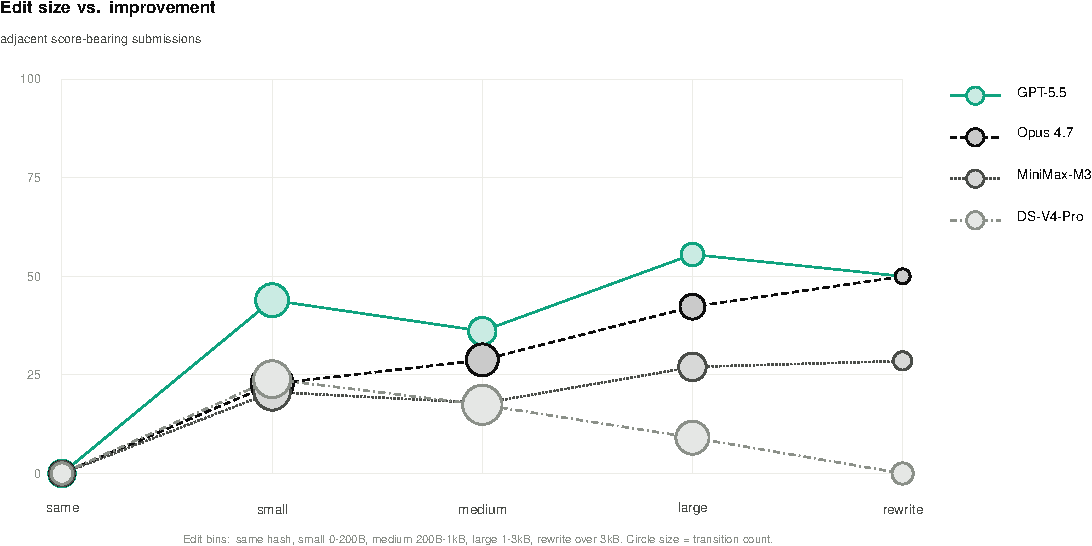
\includegraphics[width=0.78\textwidth]{figs/code_edit_risk_return.pdf}
    \caption{Observed association between policy edit size and improvement
    probability across adjacent submissions. Edit bins are computed from
    checkpoint code diffs; circle size indicates the number of transitions in
    each bin. The plot is diagnostic: large edits can represent useful
    mechanism synthesis, destructive rewrites, or
    interface repair depending on the surrounding run context.}
    \label{fig:code-edit-risk-return}
\end{figure}

Same-hash transitions have zero improvement by construction, and small or
medium edits form the common local-search regime. GPT-5.5 and Claude Opus 4.7
still improve on a meaningful share of larger structural edits, which matches
their qualitative traces: both agents introduce mechanisms and then consolidate
them. MiniMax-M3 obtains some large gains from rewrites but consolidates them
less reliably, while DeepSeek-V4-Pro less often turns large edits into
validation-best checkpoints.

\section{Policy Mechanism Case Studies}
\label{app:case-study-strategies}

The quantitative diagnostics above describe aggregate behavior; this section
shows what successful submitted policies look like. Figure~\ref{fig:gpt55-racing-diagnostics-panel}
grounds the CarRacing trace in agent-visible diagnostic artifacts. The snippets
distill representative submitted policy mechanisms from checkpoint code and
nearby stream evidence, keeping the causal structure of each strategy while
omitting interface boilerplate, constants, and environment wrappers.

\begin{figure}[H]
    \centering
    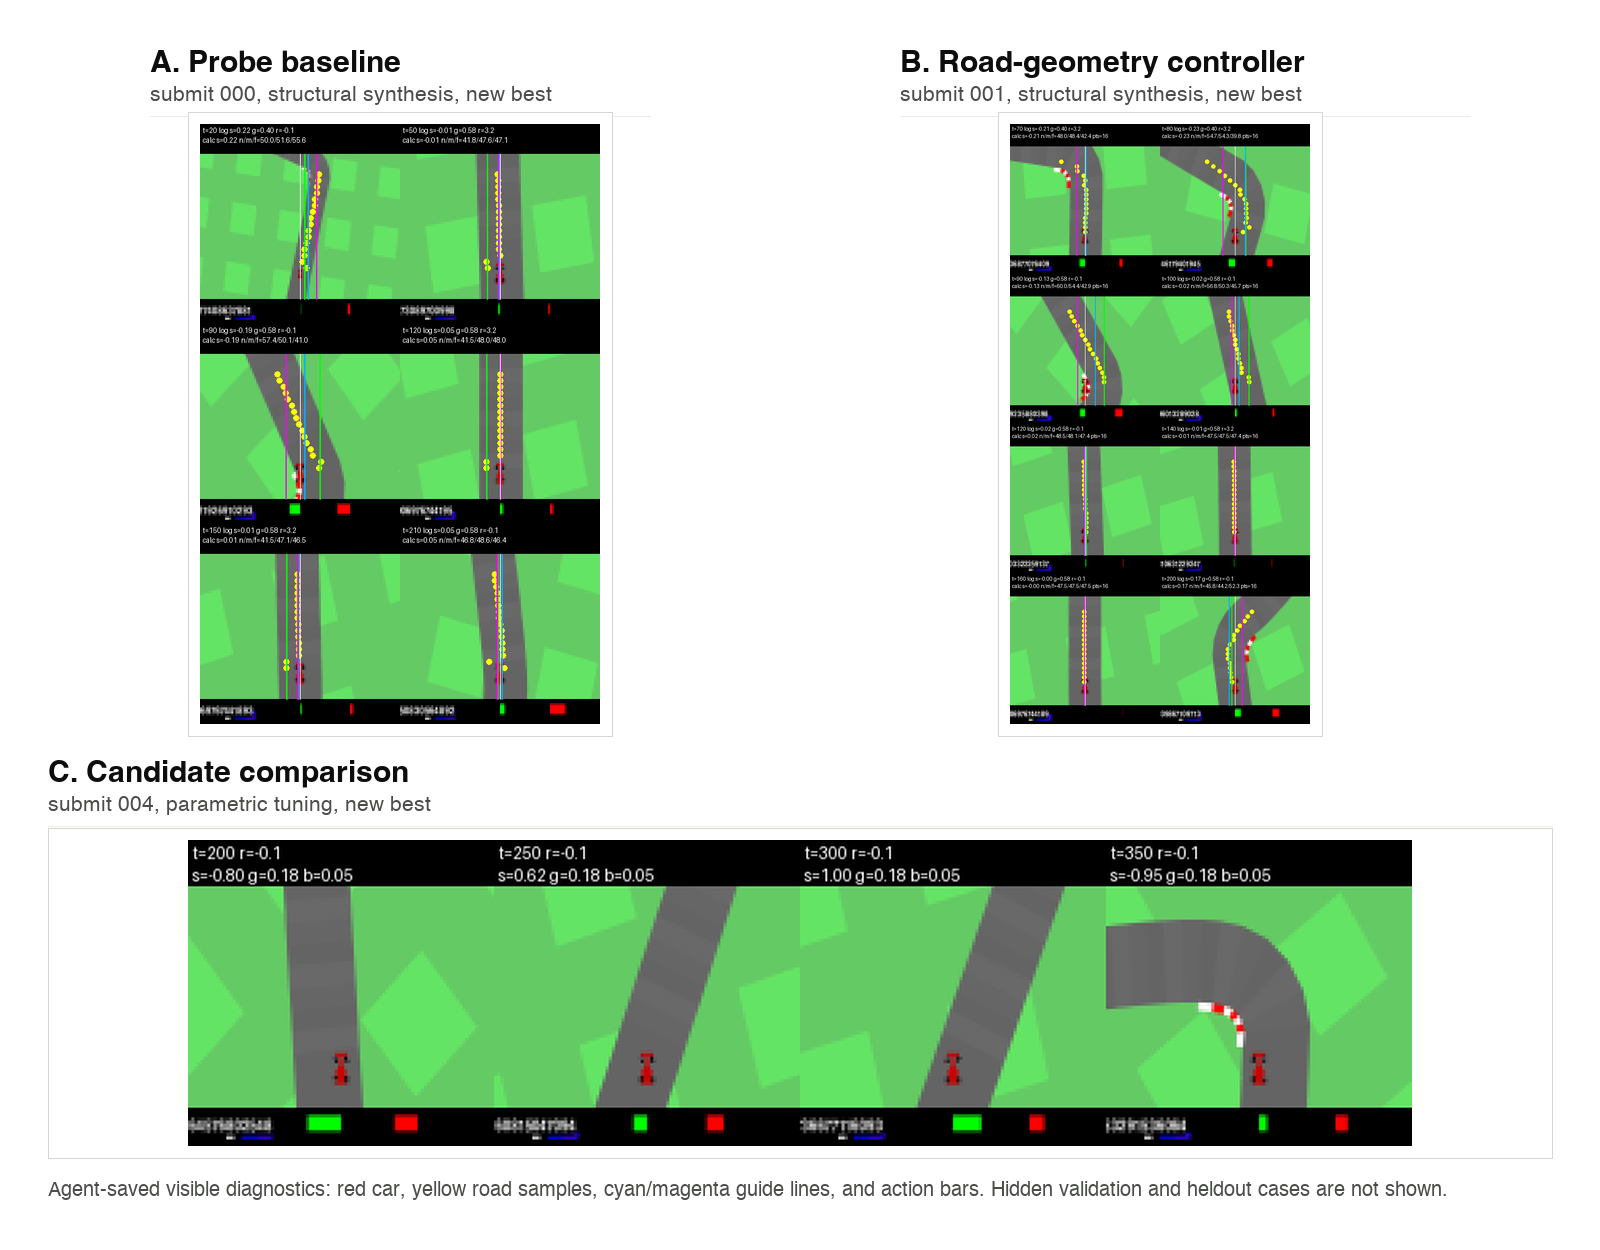
\includegraphics[width=0.98\textwidth]{figs/gpt55_racing_diagnostics_panel.png}
    \caption{GPT-5.5 CarRacing visible diagnostics saved by the agent during
    the run. Panels A--B show how structural-synthesis edits turn pixel
    observations into road-geometry control signals: yellow points mark sampled
    road evidence, cyan/magenta lines mark guide estimates, and action bars/log
    text summarize the agent's own rollout diagnostics. Panel C shows a later
    visible candidate comparison after a parametric-tuning edit. These images
    are qualitative evidence only and do not expose hidden-validation or
    held-out cases.}
    \label{fig:gpt55-racing-diagnostics-panel}
\end{figure}

\paragraph{CarRacing: road-mask lookahead and recovery.}
The strongest CarRacing policies first convert pixels into a road mask, then
trace near/mid/far centers, combine lookahead curvature with edge warnings,
and reduce speed when visual confidence drops. This turns raw frames into a
closed-loop controller with an explicit recovery mode.
\begin{strategycode}
def act(self, obs):
    centers = trace_road_centers(road_mask(obs), last_target=self.last_target)
    if not centers:
        self.lost_steps += 1
        center = global_road_center(obs)
        if center is None:
            steer = recover_toward_last_track(self.last_steer, self.last_target)
        else:
            raw = clip((center - self.center_x) / 23.0, -1.0, 1.0)
            steer = 0.45 * self.last_steer + 0.55 * raw
        self.last_steer = clip(steer, -1.0, 1.0)
        return [float(self.last_steer), 0.25, 0.0]

    near, mid, far = summarize_centers(centers)
    curvature = (far - mid) / self.width
    raw_steer = 0.75 * dev(mid) + 1.20 * dev(far) + 0.60 * curvature
    raw_steer = repair_with_global_center(raw_steer, obs, edge_alert=True)
    steer = clip(0.45 * self.last_steer + 0.55 * raw_steer, -1.0, 1.0)
    self.last_steer = steer
    self.last_target = 0.25 * near + 0.40 * mid + 0.35 * far

    turn = max(abs(steer), abs(raw_steer), abs(dev(far)))
    gas, brake = speed_schedule(turn)
    return [float(steer), float(gas), float(brake)]
\end{strategycode}

\paragraph{HalfCheetah: periodic gait with safety scaling.}
HalfCheetah exposes open-loop synthesis: agents search for a compact
oscillatory gait, then wrap it with clipping and posture-based amplitude
scaling. The policy system stores the gait parameters, and visible returns
tune phase, amplitude, and frequency.
\begin{strategycode}
def act(self, obs):
    root_height = float(obs[ROOTY])
    excess = max(0.0, abs(root_height) - self.safety_thresh)
    scale = max(self.safety_floor, 1.0 - excess)

    phase = 2.0 * math.pi * self.freq * self.t * self.dt
    hip = self.hip_amp * math.sin(phase)
    knee = self.knee_amp * math.sin(phase + math.pi / 2.0)
    ankle = self.ankle_amp * math.sin(phase + math.pi)
    action = np.array([
        hip,
        knee,
        ankle,
        -0.8 * hip,
        -0.7 * knee,
        -0.5 * ankle,
    ], dtype=np.float32)

    self.t += 1
    return np.clip(scale * action, self.action_low, self.action_high)
\end{strategycode}

\paragraph{ObstructedMaze: egocentric mapping and BFS planning.}
Successful MiniGrid policies build a persistent symbolic world model from the
7-by-7 egocentric image, update pose using previous actions, and plan toward
task objects with key, door, and blocker state. The same planner supports
frontier exploration, door toggling, pickup, drop, and obstacle clearing.
\begin{strategycode}
def act(self, obs):
    image = obs["image"]
    self.sync_pose(obs["direction"], self.last_action, self.last_front)
    self.update_world_from_view(image, pose=self.pose)
    front = self.cell_in_front(image)

    if self.target_ball_visible(front):
        action = PICKUP
    elif self.carrying_is_obstacle():
        action = self.drop_at_safe_cell(front)
    elif self.carrying_is_key() and self.door_blockers(self.key_color):
        action = self.clear_blocker_before_door(front)
    else:
        targets = (self.ball_targets() or self.key_targets()
                   or self.door_targets() or self.blocker_targets()
                   or self.frontier_targets())
        path = bfs(self.world, self.pose, targets, can_enter=self.can_enter)
        action = self.follow(path) if path else self.unstick_action()

    self.last_action = action
    self.last_front = front
    return action
\end{strategycode}

\paragraph{FetchPush: geometry-based phase controller.}
FetchPush policies compute the push direction from object to goal, move the
gripper behind the object, lower to a pushing height, and drive through the
object toward a point beyond the goal. Later repairs add a clearance phase for
cases where the gripper starts on the wrong side of the object.
\begin{strategycode}
def act(self, obs):
    raw = obs["observation"]
    grip = raw[0:3]
    obj = obs.get("achieved_goal", raw[3:6])
    goal = obs["desired_goal"]

    direction = unit(goal[:2] - obj[:2])
    distance_xy = norm(goal[:2] - obj[:2])
    behind = obj[:2] - 0.065 * direction
    along = dot(grip[:2] - obj[:2], direction)
    lateral = cross2(grip[:2] - obj[:2], direction)

    push_z = obj[2] + 0.018
    approach_z = obj[2] + 0.075
    clear_z = obj[2] + 0.115
    needs_clear = distance_xy < 0.130 and abs(lateral) < 0.045 and along > -0.020

    if distance_xy < 0.050:
        target, gains = [grip[0], grip[1], obj[2] + 0.095], (0.0, 12.0)
    elif needs_clear and grip[2] < clear_z - 0.025:
        target, gains = [grip[0], grip[1], clear_z], (0.0, 14.0)
    elif norm(behind - grip[:2]) > 0.030:
        target, gains = [behind[0], behind[1], approach_z], (20.0, 12.0)
    elif abs(grip[2] - push_z) > 0.022:
        target, gains = [behind[0], behind[1], push_z], (16.0, 16.0)
    else:
        target = [goal[0] + 0.075 * direction[0],
                  goal[1] + 0.075 * direction[1], push_z]
        gains = (22.0, 12.0)

    return servo_to_target(grip, target, xy_gain=gains[0], z_gain=gains[1])
\end{strategycode}

Across the four examples, the useful policies are small stateful programs:
they build a task abstraction, attach a controller or planner to it, and add
recovery logic for the failure modes exposed by visible feedback. This pattern
is the mechanism-level counterpart of the synthesis and tuning behavior in the
main analysis.
